\documentclass[12pt,a4paper]{article}
%\usepackage[left=0.8in,right=0.8in,top=1in,bottom=1in]{geometry}

\usepackage[superscript,biblabel]{cite}
\usepackage[parfill]{parskip}
% \usepackage{microtype} \hyphenpenalty=750

\usepackage{gensymb}

\usepackage[pdftex]{graphicx}
\usepackage{epstopdf}
% \DeclareGraphicsRule{.tif}{png}{.png}{`convert #1 `dirname #1`/`basename #1 .tif`.png}
\usepackage[utf8]{inputenc}
\usepackage{booktabs}
\usepackage[english]{babel}
\usepackage{siunitx} \sisetup{range-phrase=--,range-units=single}
\usepackage[colorlinks]{hyperref}
\usepackage{caption} \captionsetup{labelfont={sf,bf}, size=footnotesize}

% set format of document title
\usepackage{titling}
\pretitle{\begin{center}\Large\bfseries} \posttitle{\end{center}\vspace{1em}}
\preauthor{\begin{center}\large} \postauthor{\end{center}\vspace{1em}}
\predate{\begin{center}\large} \postdate{\end{center}\vspace{1em}}
\pretitle{\begin{center}\Large\bfseries} \posttitle{\end{center}\vspace{1em}}

% set formats of section headings
\usepackage[explicit]{titlesec}
\titleformat{\title}{\centering}{\thesection.}{0.5em}{\MakeUppercase{#1}}
\titleformat{\section}{\centering}{\thesection.}{0.5em}{\MakeUppercase{#1}}
% \titleformat{\section}{}{\thesection.}{0.5em}{\MakeUppercase{#1}}
%\titleformat{\subsection}[runin]{\slshape}{\thesubsection.}{0.5em}{#1. }
\titleformat{\subsection}{\slshape}{\thesubsection.}{0.5em}{#1 }
\titleformat{\subsubsection}[runin]{\slshape}{\thesubsubsection.}{0.5em}{#1. }
 
\usepackage[T1]{fontenc}
\usepackage[scaled=.90]{helvet} \renewcommand{\familydefault}{\sfdefault} \usepackage[helvet]{sfmath}

\sisetup{detect-all} % tell siunitx to detect font stuff
 
\setlength{\columnsep}{0.75cm} 

\graphicspath{{figures/}}

\providecommand{\figr}[1]{Fig.~\ref{fig:#1}}
\providecommand{\figlabel}[1]{\label{fig:#1}}
\providecommand{\tabl}[1]{Tab.~\ref{tab:#1}}
\providecommand{\tablabel}[1]{\label{tab:#1}}
\providecommand{\sectn}[1]{Sec.~\ref{sec:#1}}
\providecommand{\seclabel}[1]{\label{sec:#1}}

\providecommand{\inductor}[1]{L\textsubscript{#1}}
\providecommand{\capacitor}[1]{C\textsubscript{#1}}
\providecommand{\resistor}[1]{R\textsubscript{#1}}

% \interfootnotelinepenalty=10000

\title{The Open Source Monkey Coffin Loudspeaker}
% \author{The OSMC design team}
\author{Matthias Brennwald}
\date{\today}

\begin{document}


\maketitle

\vspace{0.2\textheight}

\section*{Important Notes and Disclaimers}
This document describes the design of the Open Source Monkey Coffin (OSMC) loudspeaker, which was developed in an ``open-source project''\cite{osmc_p1}. The aim of this project is to provide the OSMC design to DIYers for their own private purposes, for example to build a copy of the OSMC. Do not use the information developed in this project on a larger scale without written permission (for example by selling speakers based on the OSMC design or substantial parts of it).\par

The OSMC development was financially supported by diyAudio members LORDSANSUI, Paul Vancluysen, George Wright, KaffiMann, Charles Bueche, zimmer64, John Barbor, mbrennwa, and other anonymous members. Thank you!

\clearpage

\section{Overview}
The Open Source Monkey Coffin (OSMC) loudspeaker was developed by members of the diyAudio internet forum\cite{osmc_p1}. The motivation for developing this loudspeaker emerged from two diyAudio threads discussing the idea of ``open source'' loudspeaker designs\cite{osproj1_p1,osproj2_p1}. Once the types of loudspeakers that would appeal to many novice DIYers were identified, the design targets for the OSMC were defined as follows:

\begin{itemize}
\item The OSMC must be straight forward to make for DIY novices.
\item The box format should follow the ``large monitor'' format, sometimes also referred to as ``monkey coffin'' (hence the name).
\item The OSMC should be ``amplifier friendly''. It should work well with small amplifiers like the popular Amp-Camp-Amp, tube amps, etc.
\item The internal volume should not be larger than \SIrange{60}{80}{L}.
\item The OSMC should be a three way loudspeaker.
\item Keeping part costs low is not of paramount priority. If the right parts cost a lot of money and there are no cheaper equivalents, it's okay to use those parts in the design.
\end{itemize}

\clearpage

The discussions on the diyAudio forum led to the following approach to implement the OSMC:
\begin{enumerate}

\item The enclosure must be a simple rectangular box which is easy enough to make on a kitchen table.

\item For ``amplifier friendliness'', the targeted loudpseaker efficiency is \SI{92}{dB-SPL} at a distance of \SI{1}{m} and \SI{2.83}{V} input voltage, with bass extension to 45 Hz (\SI{-3}{dB}). The impedance curve must not exhibit any sharp peaks or dips, and the OSMC should qualify as an ``\SI{8}{$\Omega$} speaker''. Given the above box-size constrains, it will be challenging to achieve these targets.

\item High-quality drivers and parts should be chosed based on the technical specations required for the OSMC design. The look of the drivers has to be ``right'' for a HiFi system in a home environment (people may not want to build a speaker that looks unusual), but is second priority after the techincal specifications.

\item The woofer will determine the compromise between box size, bass-extension, and efficiency. A 10" or 12" woofer will be required.

\item The midrange driver needs to keep up with the SPL and impedance requirements. The Volt VM752 dome driver will work very well from \SI{400}{Hz} up to about \SI{3}{kHz}. While there may be other midrange drivers that could be used, the VM752 was chosen due to the general interest for this driver and because some of the OSMC designers had good experience using this driver.

\item The tweeter also needs to keep up with the SPL and impedance requirements. Classical dome or ring radiator tweeters seem to be favoured by the OSMC designers. Also, the use of a waveguide seems favourable in order to match the dispersion of the tweeter to the midrange, to reduce the effects of baffle diffraction, to increase the on-axis efficiency, and to reduce non-linear distortion of the tweeter.

\item The cross over filters will be implemented as passive circuits using steep filters in order to achieve small overlaps between the drivers in the crossover frequency bands, which reduces acoustic interferences between the drivers.

\end{enumerate}


\section{System Design}

The design process is fully documented in the diyAudio thread. The most relevant data from measurements and simulations are available in the OSMC data repository\cite{osmc_datarepo}.

\subsection{Choice and Description of Drivers}

*** Describe drivers, and why they were chosen


\subsection{Baffle and Enclosure}

*** baffle geometry (mainly deteremined by the space required for the drivers)

*** driver positions (tweeter and mid positions optimized to spread effects of diffraction at baffle edgeds over wide frequency band as much as possible; guided by golden ratio distances of driver centers relative to baffle edges)

*** bass tuning: box volume and port dimensions

*** port location (rear vs front, bottom vs centered in box, discuss pro/contra, can use any of the two options without modifying the crossover)


\subsection{Driver Measurements}\seclabel{driver_measurements}

*** Present data of raw drivers mounted in box as used for input to Vituix CAD + LEAP

*** driver impedance curves:
See \figr{impedance_curves_drivers}
Use for crossover modelling.
Discuss bass tuning.

\begin{figure}[tbp]
	\centering
	% \vspace{-10ex}
	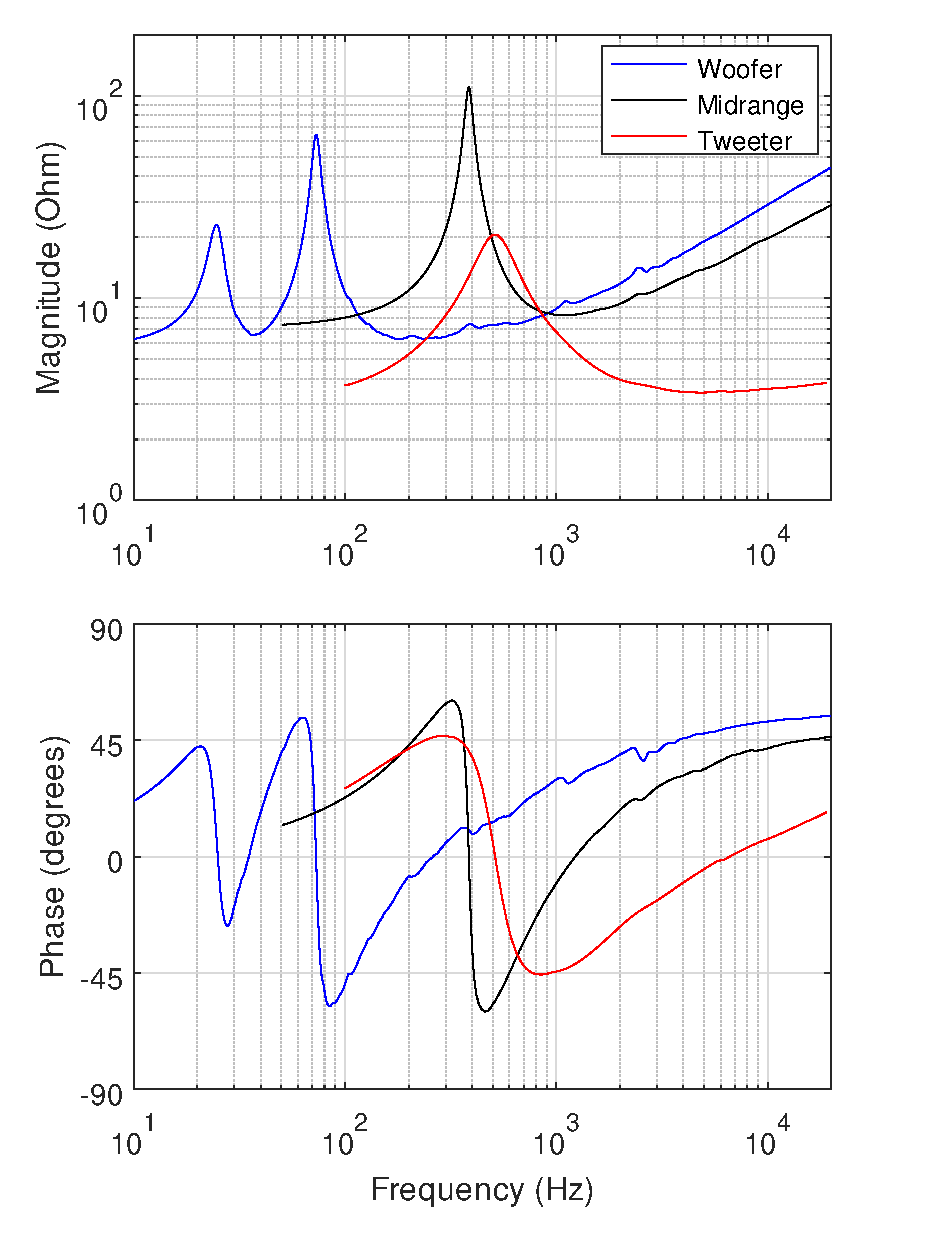
\includegraphics[width=0.7\textwidth]{impedance_curves_drivers.eps}
	\caption{Impedance curves of the drivers mounted in the OSMC box (magnitude and phase).}
	\figlabel{impedance_curves_drivers}
\end{figure}



% *** anechoic response of drivers, on axis and off-axis:
The SPL response curves of the raw drivers mounted in the OSMC box\cite{osmc_p568,osmc_p576} are shown in \figr{SPL_curves_raw}. These curves were obtained from gated impulse-response measurements, which yielded the anechoic SPL response above \SI{300}{Hz}. Measurements were taken at horizontal angles from \SI{-90}{\degree} to \SI{+90}{\degree} at \SI{15}{\degree} steps. The low-frequency parts of each SPL curve were calculated from the Thielle-Small parameters of the drivers (using LEAP)\cite{osmc_p511} and a diffraction model of the Monkey Coffin baffle (using Vituix CAD)\cite{osmc_p555}. The anechoic part and the low-frequency part of each SPL curve were merged using a ``soft splice'' in the frequency range where both parts of the curve overlapped consistently\cite{osmc_p568}. Finally, the phase response (not shown in \figr{SPL_curves_raw}) was determined by calculating the minimum phase from each of the merged SPL curves.% These SPL and phase data will be used for acoustical modelling of the OSMC system.

\begin{figure}[p]
	\centering
	\vspace{-10ex}
	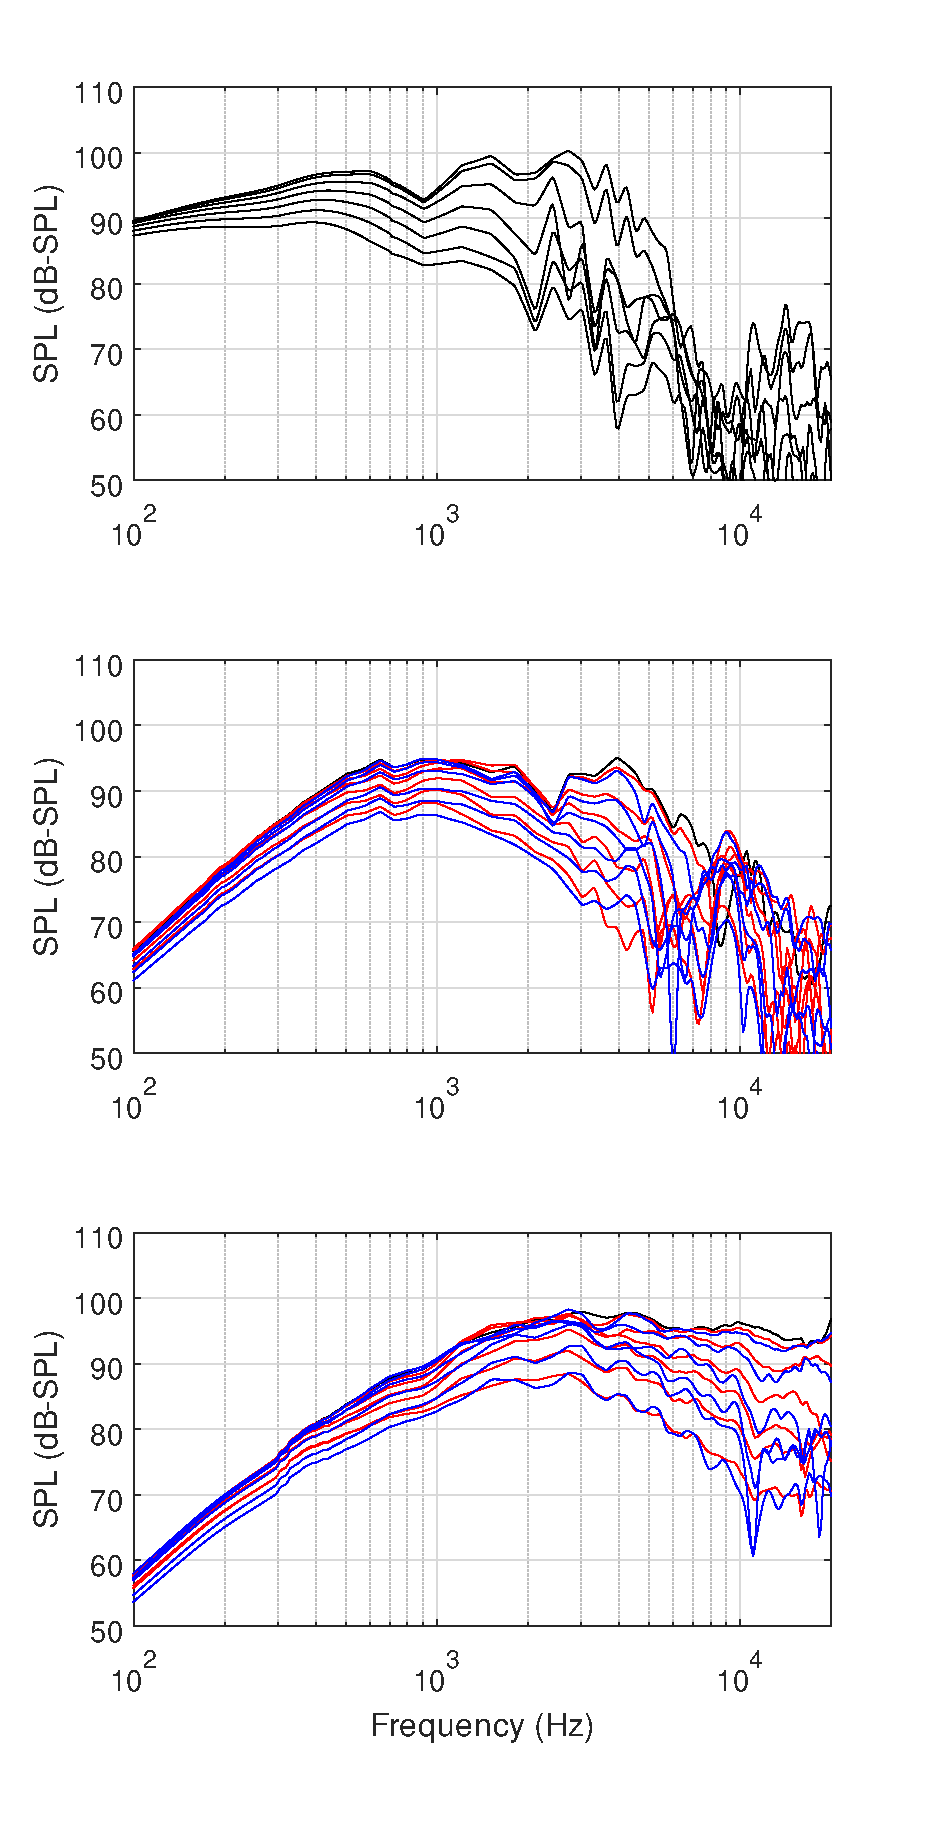
\includegraphics[width=0.7\textwidth]{SPL_curves_raw.eps}
	\caption{SPL response curves of the woofer (Faital 12PR320, top), midrange driver (Volt VM752, center) and tweeter (Scan Speak R2904/7000 with WG148 wave\-guide) mounted in the Monkey Coffin prototype box, measured at \SI{2.83}{Vrms} and \SI{1}{m} distance from the drivers, on axis and at $\pm$15\degree, $\pm$30\degree, $\pm$45\degree, $\pm$60\degree, $\pm$75\degree and $\pm$90\degree horizontal angles (symmetric for the woofer, midrange and tweeter: red curves are ``inside'' the stereo triangle, blue is ``outside''). Above \SI{300}{Hz}, the curves show the anechoic response as obtained from gated impulse-response measurements. The anechoic curves were extrapolated to lower frequencies by splicing them with modelled low-frequency curves (see text).}
	\figlabel{SPL_curves_raw}
\end{figure}



*** woofer nearfield response
Discuss box tuning





\subsection{Crossover Network}

Different filter types were considered for the OSMC. It was generally agreed to use steep filter slopes in order to achieve small overlaps between the drivers in the cross-over frequency bands with the aim of minimising acoustic interferences between the drivers.

Two different filter prototypes\cite{osmc_p685} were modelled with loudspeaker CAD tools (LEAP, Vituix CAD) using the measured electro-acoustic characteristics of the drivers mounted in the OSMC enclosure (\sectn{driver_measurements}). The first prototype uses elliptic filters, which are not very widely used in conventional loudspeaker designs. While the transfer functions of elliptic filters may exhibit some ripple near their cut-off range, they allow very steep slopes. The second prototype was designed with simpler and more conventional circuit topology using series inductors and parallel capacitors for the low-pass sections, and vice-versa for the the high-pass sections. Both prototypes were optimized for smooth and flat overall system SPL response, smooth dispersion and power response, and symmetric acoustic filter slopes near the cross-over points. The summed SPL curves of the prototype models were virtually identical.

*** INSERT VITUIX GRAPHS HERE (FOR BOTH PROTOTYPES)

For testing purposes, both filter prototypes were implemented in a miniDSP digital signal processor using infinite-implulse-response (IIR) filters. Listening tests showed that both filter prototypes resulted in very similar overall sound. After long listening tests, however, the elliptic filter was preferred because it sounded slightly more transparent\cite{osmc_p708}. The elliptic filter topology was therefore used for further development of the OSMC cross-over filters. Several iterations of CAD models, DSP filters, acoustic measurements, and listening tests. The schematic of the final cross-over filters is shown in \figr{OSMC_EL_xover_schem}.

\begin{figure}[p]
	\centering
	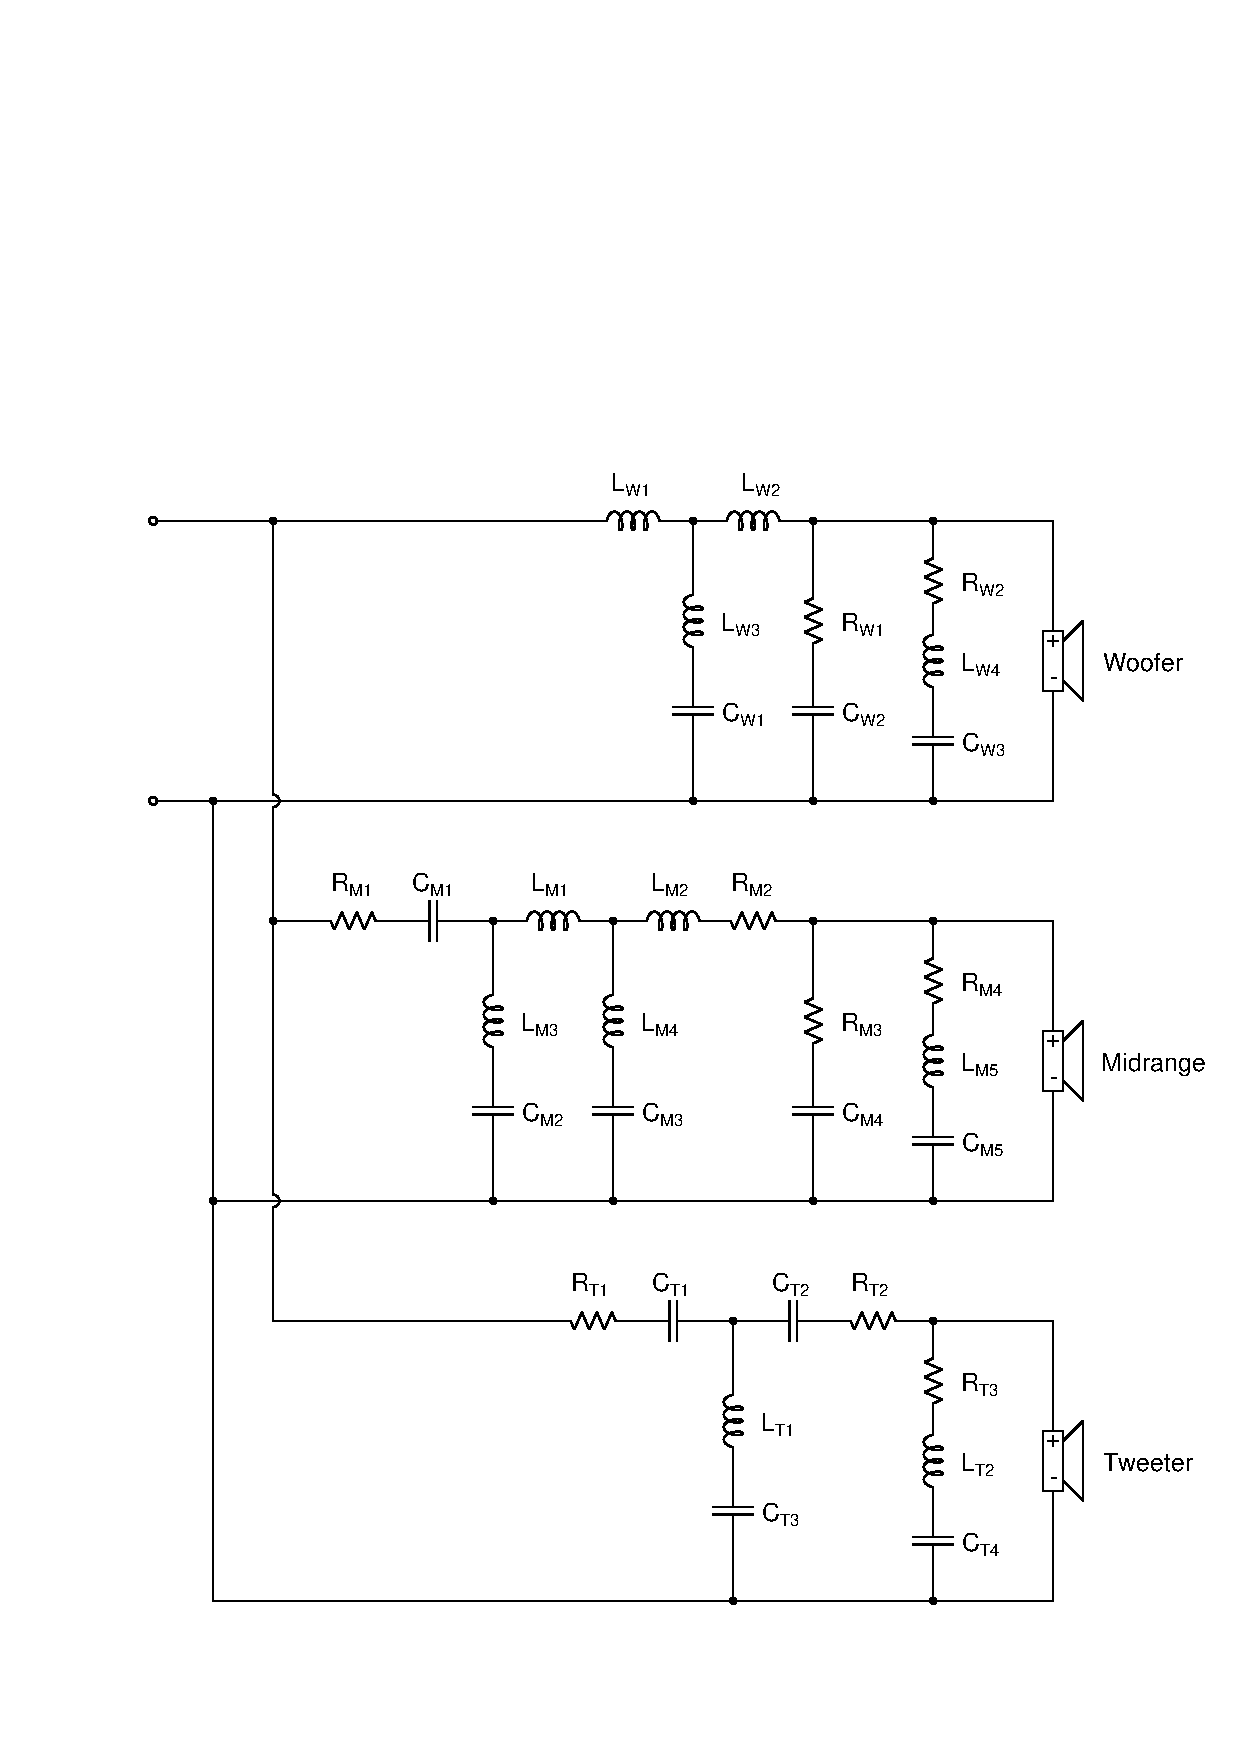
\includegraphics[width=\textwidth]{EL34_20190303.pdf}
	\caption{OSMC cross-over filters (elliptic)}
	\figlabel{OSMC_EL_xover_schem}
\end{figure}

\begin{table}[tb]

\centering
\caption{List of parts in \figr{OSMC_EL_xover_schem}.}
\footnotesize
\tablabel{tab:OSMC_EL_xover_parts}
\begin{tabular}{ccp{0.68\textwidth}} 
\toprule
Part & Value & Description\\ 
\midrule 
% \multicolumn{3}{c}{Woofer filter}\\
% \midrule

% woofer parts
\inductor{W1}	& \SI{6.8}{mH} / \SI{0.19}{\ohm}	& Laminated iron core (e.g.~Mundorf BS180, Feron, I core, baked varnish)\\
\inductor{W2}	& \SI{1.8}{mH} / \SI{0.09}{\ohm}	& Laminated iron core (e.g, Mundorf BS180, Feron, I core, baked varnish)\\
\inductor{W3}	& \SI{0.1}{mH} / \SI{0.23}{\ohm}	& Air core (e.g.~Mundorf BL71, baked varnish)\\
\inductor{W4}	& \SI{15}{mH}  / \SI{1.12}{\ohm}	& Iron core (e.g, Mundorf BH71, Ferrite, baked varnish)\\
\capacitor{W1}	& \SI{118}{\micro F}			& Parallel combination of \SI{100}{\micro F} bipolar electrolytic and \SI{18}{\micro F} MKP (e.g.~Mundorf ECAP50-100 and MCAP250-18)\\
\capacitor{W2}	& \SI{33}{\micro F}			& Bipolar electrolytic (e.g.~Mundorf ECAP70-33)\\
\capacitor{W3}	& \SI{267}{\micro F}			& Parallel combination of \SI{220}{\micro F} and \SI{47}{\micro F} bipolar electrolytics (e.g.~Mundorf ECAP63-220 and ECAP50-47)\\
\resistor{W1}	& \SI{6.8}{\ohm} / \SI{10}{W}		& MOX type (e.g.~Mundorf MR10-6.80)\\
\resistor{W2}	& \SI{5.6}{\ohm} / \SI{10}{W}		& MOX type (e.g.~Mundorf MR10-5.60)\\

\midrule

% midrange parts
\inductor{M1}	& \SI{1.2}{mH} / \SI{0.39}{\ohm}	& Air core (e.g.~Mundorf BL125, baked varnish)\\
\inductor{M2}	& \SI{0.33}{mH} / \SI{0.15}{\ohm}	& Air core (e.g.~Mundorf BL100, baked varnish)\\
\inductor{M3}	& \SI{6.8}{mH} / \SI{0.46}{\ohm}	& Iron core (e.g.~Mundorf BH100, Ferrite, baked varnish)\\
\inductor{M4}	& \SI{0.12}{mH} / \SI{0.15}{\ohm}	& Air core (e.g.~Mundorf BL100, baked varnish)\\
\inductor{M5}	& \SI{2.7}{mH} / \SI{1.01}{\ohm}	& Iron core (e.g.~Mundorf BP71, Ferrite, baked)\\
\capacitor{M1}	& \SI{33}{\micro F}			& MKP (e.g.~Mundorf MCAP250-33)\\
\capacitor{M2}	& \SI{267}{\micro F}			& Parallel combination of \SI{220}{\micro F} bipolar electrolytic and \SI{47}{\micro F} MKP (e.g.~Mundorf ECAP63-220 and Mundorf MCAP250-47 (MKP)\\
\capacitor{M3}	& \SI{6.8}{\micro F}			& MKP (e.g.~Mundorf MCAP250-6.80)\\
\capacitor{M4}	& \SI{4.7}{\micro F}			& MKP (e.g.~Mundorf MCAP250-4.70)\\
\capacitor{M5}	& \SI{68}{\micro F}			& Bipolar electrolytic (e.g.~Mundorf ECAP50-68)\\
\resistor{M1}	& \SI{2.7}{\ohm} / \SI{10}{W}		& MOX or wire wound (non-inducitve) (e.g.~Mundorf MRES20-2.7)\\
\resistor{M2}	& \SI{5.6}{\ohm} / \SI{10}{W}		& MOX or wire wound (non-inducitve) (e.g.~Mundorf MRES20-5.6)\\
\resistor{M3}	& \SI{8.2}{\ohm} / \SI{10}{W}		& MOX or wire wound (e.g.~Mundorf MR10-8.2)\\
\resistor{M4}	& \SI{8.2}{\ohm} / \SI{10}{W}		& MOX or wire wound (e.g.~Mundorf MR10-8.2)\\

\midrule

% tweeter parts
\inductor{T1}	& \SI{0.22}{mH} / \SI{0.38}{\ohm}	& Air core (e.g.~Mundorf BL71, baked varnish)\\
\inductor{T2}	& \SI{0.47}{mH} / \SI{0.64}{\ohm}	& Air core (e.g.~Mundorf BL71, baked varnish)\\
\capacitor{T1}	& \SI{4.7}{\micro F}			& MKP (e.g.~MCAP250-4.7)\\
\capacitor{T2}	& \SI{15}{\micro F}			& MKP (e.g.~MCAP250-15)\\
\capacitor{T3}	& \SI{100}{\micro F}			& Parallel combination of \SI{82}{\micro F} bipolar electrolytic and \SI{18}{\micro F} MKP (e.g.~Mundorf ECAP50-82 and MCAP250-18)\\
\capacitor{T4}	& \SI{100}{\micro F}			& Bipolar electrolytic (e.g.~Mundorf ECAP50-100)\\
\resistor{T1}	& \SI{3.9}{\ohm} / \SI{10}{W}		& MOX or wire wound (non-inducitve) (e.g.~Mundorf MRES20-3.9)\\
\resistor{T2}	& \SI{1.0}{\ohm} / \SI{10}{W}		& MOX or wire wound (non-inducitve) (e.g.~Mundorf MRES20-1.0)\\
\resistor{T3}	& \SI{4.7}{\ohm} / \SI{10}{W}		& MOX type (e.g.~Mundorf MR10-4.7)\\
\bottomrule
\end{tabular}
\end{table}


\subsection{System performance}

*** SPL curves of full system (on-axis padded with near-field bass, off-axis)

*** Impedance curve

*** How does the result compare to the build targets?


\section{Construction}

\subsection{Baffle and Enclosure}

*** Routing irregular drivers\cite{reddit_flushmount}

*** BRACING

*** DAMPING


\subsection{Fitting the Waveguide}

*** WG148: machining

*** augerpro version: ...


\subsection{Cross Over Filters}

*** how to (not) construct the filters

*** possible modifications (better parts, other part values: use Vituix CAD to see effects)


% list of references
\bibliographystyle{unsrt}
\bibliography{osmc_refs}


\end{document}
